%\documentclass[paper]{geophysics}
\documentclass[manuscript,revised]{geophysics}
%\documentclass[twocolumn,revised]{geophysics}

% An example of defining macros
\newcommand{\rs}[1]{\mathstrut\mbox{\scriptsize\rm #1}}
\newcommand{\rr}[1]{\mbox{\rm #1}}

\newcommand{\psm}{\textit{PSM} }
\newcommand{\twod}{2-D }
\newcommand{\thrd}{3-D }
\newcommand{\bialt}{\textit{BiAlt} }

\usepackage{lineno}

% printing options
%\usepackage{pgfpages}
%\pgfpagesuselayout{4 on 1}[letterpaper,border shrink=5mm]


\begin{document}

\title{Refined experimental studies for improving the reduced-scale physical modeling of seismic subsurface measurement}

\renewcommand{\thefootnote}{\fnsymbol{footnote}} 

\ms{version 1.0} % manuscript number

\address{
\footnotemark[1]LUNAM-IFSTTAR, \\
\footnotemark[2]OSUNA \\
\footnotemark[1]LPGN, \\}
\author{Damien Pageot\footnotemark[1]\footnotemark[2], Donatienne Leparoux\footnotemark[1], Mathieu Le Feuvre\footnotemark[1], Olivier Durand\footnotemark[1] and Yann Capdeville\footnotemark[3]}

\footer{Example}
\lefthead{Dellinger \& Fomel}
\righthead{\emph{Geophysics}}

\maketitle

\begin{abstract}

\noindent The potential of experimental seismic modeling at reduced scale is explored since several years because it provides an intermediate step between numerical tests and geophysical campaigns on field sites. In this scope, among the experimental benches using laser interferometry for recording ultrasonic data, the MUSC system is designed as a reliable tool, able to produce experimental seismic reduced scale data from setup involving multi-sources and multi-receivers positions. The recorded signals contain the complete field suitable for high-resolution imaging techniques like Full Waveform Inversion. However, experimental seismic modeling uses a point-source and generates 3-D seismic data whereas most of wave propagation and imaging algorithms make use of \twod forward modeling for numerical cost reasons. Further, geometrical spreading corrections applied on \thrd data are limited when geological structures become complex. This leads to inaccurate relative amplitudes between wavefronts which can have an important impact on the quality of the recovered model of parameters. High-resolution imaging methods like FWI are also sensitive to the source waveform and the initial synthetic source must be, as the initial model, close enough to the true one. During the inversion process, the source wavelet can be estimated, per shot or for the whole dataset, but is strongly dependent of the initial model for inversion, \textit{i.e.}, the estimated source will absorb inaccuracy of the initial model and the of update models. It results in ill-reconstruction of geological structures and parameter values. In this paper we seek to show the capacity of the experimental seismic modeling, like it is involved in the MUSC system, to generate reproducible, realistic and suitable data which can be used as reference for \twod high-resolution imaging method validations. In this scope, with the support of \twod and \thrd numerical modeling algorithm bsed on the Spectral Element Method, we have first refined the comparison between numerical and experimental data by generating accurate experimental line-sources (\twod) which allow to avoid geometrical spreading correction of \thrd data. By this approach, we have shown the relevance of this step compared to corrections methods designed to 3D data and found in the litterature, particularly when all the arrivals (surface waves and reflected body waves) need to be taken into account. Second, we have assessed the stability and the reproducibility of the source emitted in a model by the piezoelectric transducer during a campaign involving multi-sources multi-receivers acquisitions. The results of the source estimation through the 2D and 3D experimental setups as well as the reproducibilty of the wave-shape contribute to refine the validation of the multi-source and multi-receiver measurement bench as an experimental seismic reduced scale modeling system and prove the capacity of ultrasonic devices used, associated to the positionnment bench to perfectly and quantitatively reproduce the seismic surface measurements and the complete wave-field involved.
\end{abstract}

\modulolinenumbers[5]
\linenumbers

% ## INTRODUCTION
\section{Introduction}

% #### Nature and scope of the problem

\noindent Since the early developments of seismic imaging methods in the middle of 20th century, several approaches and algorithms innovations are still proposed in current research projects. The improvements deal with both the qualitative imaging techniques like migration (e.g. \citet{Berkhout_MSS_2012,Guofeng_GPU_2013}), novel applications of quantitative imaging methods such as the first arrival tomography (e.g. \citet{Bohm_CWS_2015}), or even more recent approaches like the Full Waveform Inversion (e.g. \citet{Perez_AWI_2014}, see \citet{Virieux_FWI_2009} for a revue of this last decade). The refinements are proposed for different scales like near surface applications for civil engineering topics or more deeper investigation for example for oil prospection or crustal imaging at regional or global scales. They are mostly validated by using synthetic data, for example with well known shared benchmark (like the Marmousi case). However, the synthetic data are generally computed using the same wave propagation modeling engine used in the inverse problem process. In other terms, the synthetic data are computed with some assumptions which are the same in the inverse problem, for example the approximation of acoustic propagation, a 2D space medium, or a 2D line source. This approach, called \textit{inverse crime} \citep{Wirgin_TIC_2004} is particularly useful for validating an algorithm in its early development stage but does not take into account the artifacts that can be due to the assumptions of the forward problem. Some authors tackle this issue by providing 3D data which are inverted with a 2D approach or other restrictive assumptions (e.g ). But also in this case, the approach does not allow to assess the efficiency of the method for real seismic data. Moreover, because no one knows precisely the Earth interior, it is difficult to evaluate the capacity of a method to recover physical parameters and structures from real seismic data which can lead sometimes to geological misinterpretation due to numerical artifacts \citep{Morozov_ARF_2004}. Thus, it is necessary to add a step for which imaging methods will be tested for experimental seismic measurements obtained under controlled conditions.

% ## \noindent The best way to satisfy this need is to use Physical Small Scale Modeling Methods (noted \psm subsequently). \psm were used since several years to study the propagation of waves in various media with several stage of complexity, from acoustic wave propagation in homogeneous media to elastic wave propagation in \thrd heterogeneous anisotropic media \citep{Rieber_EWP_1936,Howes_SMS_1953,Hilterman_TDM_1970,French_MRP_1974,Bishop_LVM_1985,Pratt_FWI_1999,Favretto_NMT_2013,Sarkar_TPM_2003,Isaac_SMS_1999}, and allow to generate experimental seismic data under well-controlled conditions. In this way, recent studies have been conducted to simulate multi-sources and multi-receivers through piezo-electric transducers \citep{Wong_SPM_2009}. An alternative approach consists in using the laser interferometry as the receiver system, as done in the MUSC Laboratory \citep{Bretaudeau_SSA_2008b,Bretaudeau_SSM_2011,Bretaudeau_FWI_2013}, \textit{Mesure Ultrasonore Sans Contact} in French. This technology, by avoiding the contact of the receivers on the model, allows to by-pass the coupling issue of transducers that is difficult to model. In this way, the MUSC laboratory is designed to simulate (1) wide-angle on-shore acquisitions modeling both body waves and surface waves, (2) automatic multisource-multireceiver measurements with a high-productivity, (3) high-precision source-receiver positioning and (4) high-precision recording of absolute surface displacement without coupling effects. 

\noindent The best way to satisfy this need is to use Physical Small Scale Modeling Methods (noted \psm subsequently). \psm were used since several decades to study the propagation of waves in various media with several stages of complexity, from acoustic wave propagation in homogeneous media to elastic wave propagation in \thrd heterogeneous anisotropic media. The objectives of the approaches have firstly been adressed to understand the propagating waves phenomenology (for example  Rieber, Howes) and in a second period for testing imaging process (Hiltermann, French, Bishop, pratt, Isaac), or for valdating numerical tools (Favretto). For these different works, the technology used has become more and more sophisticated. Nowadays most of these benches involve piezzo-electric transducers to simulate multi-sources and multi-receivers \citep{Wong_SPM_2009} or immersed zero-offsets profiles (Favretto). An other technique recently used is based on laser interferometry for recording the seismic signal without coupling effects in solid media (Bodet, Van Wijk, Bretaudeau 2011,2013), or in gelee ( ). All these works have shown the relevance of carrying out experimental seismic data under well-controlled conditions. However key points remain crucial if we seek to quantitatively simulate the complete seismic wave field recorded in case of seismic surface measurement generated with a hammer fall source, firstly because of the presence of surface waves that avoids the possibility of using immersed media and secondly because the emitted source pattern has to be omnidirectional which implies a physical source point. In this aim, the MUSC (Mesures Ultrasonores Sans Contact in french) system has been designed  \citep{Bretaudeau_SSM_2011} to simulate (1) wide-angle on-shore acquisitions modeling both body waves and surface waves, (2) automatic multisource-multireceiver measurements with a high-productivity, (3) high-precision source-receiver positioning and (4) high-precision recording of absolute surface displacement without coupling effects. 

\noindent These abilities have been validated through a comparison of experimental data to numerical simulation in a 2-dimensions space containing a cavity \citep{Bretaudeau_SSM_2011}. The results showed very fine similarities concerning the diffracted and converted arrivals when the source waveform is taken into account. For that, the numerical source was simulated in 2D and some corrections were required to compare the amplitude results, with some remaining weak discrepancies as mentioned in the discussion of \citet{Bretaudeau_SSM_2011}. Moreover, the source diagram was assessed with a parallel measurement bench, showing an omnidirectional propagation but the repeatability of the source impact was not studied.

% #### State the objectives
\noindent Our objective here is to complete the validation of the capability of ultrasonic devices to precisely and quantitatively simulate surface seismic data carried out with multi-sources and multi-recievers setting. Thus this quantitative refined approach will increase the potential of the MUSC system as a reliable tool for generating experimental data which will be distributed in the scientific community.
\noindent In this way, we further present two studies of experimental data in order to : 1) refine the quantitative comparison between numerical and experimental data by taking into account the 3D/2D geometrical spreading effects through an alternative way that we compare to the corrections proposed in the litterature ; 2) identify the reproducibility of the source impact and, consequently, data repeatability. These approaches will complete the knowledge of the system and facilitate the achievement of massive multi-source and multi-receiver data simulating subsurface seismic experimental campaigns. Moreover, they provide quantitative informations about the data quality for geophysicists who need to use them measurement based on reduced scale models. 

% #### Describe the method of investigation
\noindent In order to achieve these objectives, we used a seismic wave modeling code based on the Spectral Element Method \citep{Komatitsch_SEM_1998,Komatitsch_ISM_1999,Komatitsch_SEM_2005,Festa_PML_2005} that allows to provide numerical signals as reference data for comparison. The Spectral Element Method (SEM) has several advantages compared to finite differences and finite elements, such as: (1) a weak formulation which can naturally take into account the free surface, (2) an explicit scheme in time domain facilitating parallelization and reducing the computational cost, (3) a spatial discretization (mesh) convenient for the representation of complex environments and (4) high precision results as well as low numerical dispersion.

% #### Describe the principal results of the investigation

\noindent The numerical characteristics of the code used are described in a first part below. Afterwards, the specificities of the MUSC system are explained, followed by the presentation of the models used. Finally The two coupled studies on experimental data are detailed, in the respective aims (1) of refining the comparison between numerical and experimental data by taking into account the geometrical spreading effects between \twod and \thrd data through an alternative way, and (2) of identifying the reproducibility of the source impact to validate the data reproducibility.


% ## METHODS
\section{Methods}

% #### Spectral Element Method
\subsection{Numerical modeling: Spectral Element Method}

\noindent Various numerical methods exist to resolve the equation of motion in arbitrary elastic media. The most widely used for seismic applications is the Finite-Differences (FD) method \citep{Virieux_PSV_1986,Levander_PSV_1988,Robertsson_FDM_1994,Pratt_EWM_1990,Stekl_VEM_1998,Saenger_FDM_2004} which estimates each derivative on a regular Cartesian grid using a Taylor development \citep{Moczo_FDM_2004} of order \textit{n}. FD is simple to implement and robust but shows some limitations. First the Cartesian grid is defined by the minimum propagated wavelength ($\lambda_{min}$) in the full medium which conducts to a very small spatial step in case of low velocities zones as it is usually the case for subsurface issues. Moreover, \citet{Saenger_FDM_2000} show that 60 points by wavelength ($\lambda$) are needed to correctly model propagation of Rayleigh wave in order $n=2$ where only 15 points by $\lambda$ are required to correctly model propagation of body waves which increases drastically the numerical cost in case of near-surface modeling experiments. Second, the Cartesian grid does not provide a suitable tool to reproduce properly complex topography and interfaces. 

\noindent To overcome this limit, one can use the Finite-Elements Method (FEM) which is another popular method used for wave propagation modeling \citep{Lysmer_FEM_1972,Seron_FEM_1990,Hulbert_FEM_1990}. FEM is based on a variational formulation of the equation of motion and gives a continuous approximate solution in space using polynomial basis functions defined on each node of each cell of the mesh. The natural boundary conditions of FEM is the free surface and the triangular (in 2D) or tetraedric (in 3D) unstructured meshes are well adapted to complex media and topography. However, low polynomial basis are inadequate with fine spatial discretization and the required discretization to obtain precise and non-dispersive solution is numerically costly. 

\noindent Parallel, at the end of the 20th century, the Spectral Element Method (SEM), widely used in fluid dynamics \citep{Patera_SEM_1984,Korczak_SEM_1986,Karniadakis_FEM_1989}, has been adapted to seismic wave propagation \citep{Komatitsch_SEM_1998,Komatitsch_ISM_1999,Komatitsch_SEM_2005,Festa_PML_2005}. The SEM is a variant of FEM based on a high-order piecewise polynomial approximation of the weak formulation of the wave equation which leads to a spectral convergence ratio as the interpolation order increases. 

\noindent In this method, the wavefield is formulated in terms of high-degree Lagrange interpolants, and the integrals calculation are based on the quadrature of Gauss-Lobatto-Legendre (gll). This combination leads to a perfectly diagonal mass matrix which provides in turn a fully explicit time scheme suitable for numerical simulations on parallel computers.

\noindent SEM inherits the flexibility and the natural free surface condition of the FEM \citep{Tromp_SEM_2008}. The typical element size $e_{s}$ that is required to generate an accurate mesh is of the order of $\lambda_{min} /2 < e_{s} < \lambda_{min}$ for order 5 and $\lambda_{min} < e_{s} < 2\lambda_{min}$ for order 9, $\lambda_{min}$ being the smallest wavelength of waves propagated in the model. In our study, the models are meshed with quadrangles (2D) and hexaedras (3D) using the open-source software package GMSH \citep{Geuzaine_MSH_2009}. It is particularly well suited to handle complex geometries and interface matching conditions \citep{Cristini_SEM_2012}. In order to simulate infinite or semi-infinite domain, SEM can use Perfect Match Layers boundary conditions \citep{Berenger_PML_1994,Festa_PML_2005}. However they are not used here because we simulate scale models which are spatially limited for the use in the MUSC system. The latter is described below in terms of technical specifications.


% #### MUSC bench
\subsection{Physical modeling: MUSC system}

\noindent The MUSC system \citep{Bretaudeau_SSA_2008b,Bretaudeau_SSM_2011,Bretaudeau_FWI_2013} is built to experimentally reproduce field seismic data with a great accuracy on reduceds scale model. Figure \ref{panel_musc_bench} recalls the measurement bench and its components : it is composed of a honeycomb tab and two arms which control the source and the receiver positions with a precision of 10 $\mathrm{\mu m}$.

\noindent The receiving system of MUSC system is a laser interferometer based on the phase shift of the reflected laser signal due to the particular displacement at the surface of the model during the seismic waves propagation in the medium. An integrated real-time calibration system enables a continuous conversion to a quantitative measure of the particular displacement. The diameter of the laser beam on the model surface equals 20 micrometers for the focal distance of 40 mm and allows a detection of a vertical displacement of the order of the nanometer in the frequency range from 10 kHz to 20 MHz. The laser interferometer constitutes a non-coupled receiver which avoids the complicated modeling of the coupling effects on measurement.

\noindent Note that using a laser source needs more security protocols in the laboratory and up to now, the seismic source in the MUSC laboratory is simulated by a piezoelectric transducer linked to a launching and synchronization system. It allows to choose the source function, i.e., a waveform like a Gauss or Ricker function, for a central frequency $f_{0}$ and a time delay $t_{0}$. For that, the source is generated by a waveform generator and is then amplified before being transmitted to the small-scale-model.

\noindent For the purpose of reduced scale modeling, the change of scale must keep the relationship between observables, i.e. amplitudes and time arrivals. Concerning the amplitude, the quality factor $Q$ will be chosen to be in the same range as the materials of near surface. For the time arrivals, the key parameter is the rate between the propagated seismic wavelength and the spatial dimensions of the experience that includes the model geometry, the spatial increment between the sources and the receivers positions, but also the dimensions of the source impact. In the framework of seismic physical modeling, this latter must be as close as possible to a point source in order to simulate the spatial energy repartition of a weight drop at the soil surface, i.e. with an isotropic directivity of the emitted P waves.

\noindent In the MUSC system, the main frequency bands used for reduced scale data are [ 20 KHz ; 200 KHz] and [ 300 KHz; 800 KHz], respectively called here "low frequency band" and" high frequency band". For the lower spectral band, a commercial piezo-electric transducer is used without any coupling gel. For the higher band, the piezoelectric source is coupled through a conical adapter which is sticked to the transducer in order to obtain the expected impact surface. The resulting source pattern is isotropic enough in the spectral band of interest (see \citep{Bretaudeau_SSM_2011} for more details).

\noindent The lower frequency band is well adapted to simulate seismic experiment applied to near surface through the scales ratios proposed in tables 1 and 2. In the first case (table 1), a central frequency of 100 KHz in the laboratory corresponds to a central frequency of 100 Hz on the field, whereas in the second one (table 2) a central frequency of 100 KHz in the laboratory corresponds to a central frequency of 50 HZ on the field. Note that with these propositions, the  quality factor $Q$ and the density $\rho$ are modeled with a ratio equal to 1, i.e. they remain the same at both of the scales. Actually small-scale models are generally made of thermoplastic or casting epoxy resin materials \citep{Bretaudeau_FWI_2013}.The mechanical properties of these materials provide attenuation characteristics close to natural soil materials of subsurface media. Their seismic velocities are about 2 times of those in subsurface materials as proposed in table 2. The possibilities of combinations can generate the impedance contrasts encountered in the geophysical issues. 

\noindent The MUSC bench presented above has been studied for simulating with a great reproducibility the typical field campaigns of subsurface seismic measurement. The validation was achieved by comparison between small scale measurement and numerical data \citep{Bretaudeau_SSM_2011}. Results have shown a great reproducibility of the converted and diffracted events recorded on the vertical component. The amplitudes analysis had been conducted through 2D-3D corrections and small discrepancies remained due to the difficulty of taking into account the S and P waves in the same way. For this reason, we propose here to refine the study by testing a more recent correction methodology \citet{Schafer_LSS_2014} as well as providing experimental and numerical, 2D and 3D data. This approach will be achieved through data carried out on two models that are presented below.


% ## Models
\subsection{Characteristics of the scale models tested}

\noindent In this study, we consider two different reduced scale models. The first one is homogeneous whereas the second one contains a deeper layer with a geometrical variation of the interface along the profile. The top layer, as well as the entire first model, is made of epoxy-resin called F50. The deeper layer is built with a more dense resin called LAB1000. The latter model is called \bialt. The specific properties of these two kinds of resins are summarized in the table 3. As required, note that the Q-factor values are of the same order of the Q-factor value in the shallowest parts of the natural media.

\noindent As described in the previous part and proposed in table 2, it is possible to take into account a scale ratio equal to 2 for the velocities, and use a 100 KHz Ricker source in order to simulate a 50 Hz Ricker source in reality. This seems realistic for simulating an hammer impact on the soil. In this case, the distance scale ratio is 1000 such that a 1 mm distance in the laboratory experiment corresponds to a 1 m distance in reality. Following these rules, we propose several shots described in the following part. 

\noindent The recorded signals will be finely analyzed for a maximum offset equal to 60 mm in the case of the homogeneous model and 100 mm for the \bialt model. Thus, the resin models have to be big enough in order to carry out this receiver-source distances without providing boundary echoes which could interfere with the direct arrivals. For that, the homogeneous model is 500 mm long and 504 mm large and 115 mm high. The \bialt model is 300 mm large and 200 mm high. The interface geometry is presented in figure 3. It simulates an interface between a 3 m thick layer of clay overcoming a limestone layer.

\noindent The numerical meshing required for numerical simulations involve dimensions of cells about $e_{s}<3.43\ mm$ for F50 material and $e_{s}<4.66\ mm$ for the LAB1000 material, considering a polynomial order $n=5$ and a maximum frequency $f_{max}=300\ kHz$. The resulting meshing structure for the \bialt model is presented figure \ref{panel_bialt_mesh}.
There is no PML in order to really simulate the reflexions due to the model boundaries.

\noindent These two resin blocks as well as their corresponding numerical models will be used for generating seismic data with punctual sources but also line sources in order to study the effective wavelet emitted in the MUSC bench and its reproducibility as described in the two next parts.

\section{Results}

% #### From point-source to line-source acquisition
\subsection{From point-source to line-source response}


\noindent The approach detailed here consists in generating data with a 2D line source as well as a 3D source point and analysing the similarity to numerical results under the same conditions. This is conducted to answer to two needs : 1) the quantitative refined validation of the reduced scale data , 2) the validation of the reduced scale data as a 2D set which is intermediate between numerical simulation and field data suitable for the 2D imagery tests . Indeed, in the framework of wave propagation modeling and imaging methods, even if \thrd acoustic algorithm exists \citep{benhadjali_FWI_2008,plessix_FWI_2010} and \thrd elastic algorithm are always in development \citep{castellanos_AMD_2011,Borisov_FWI_2015}, most of available algorithms are limited to the \twod elastic and \thrd acoustic approximation especially for computational cost causes. More, a widely used way to validate imaging methods consists in inverse crime while the validity of applications on real dataset is conditioned by strong \textit{a priori} and a weak knowledge of the target. All of these leads to a limited validation of the efficiency of imaging methods to recover parameter models. Thus, it is critical for \twod inversion of field data to accurately correct the difference between \twod and \thrd geometrical spreading.

\noindent Point-source data can be corrected from geometrical spreading using a simple two-steps signal processing: (1) convolving each trace by $\sqrt{t^{-1}}$, where $t$ is the time, to correct the phase shift of $\pi/4$ and (2) applying a taper $\sqrt{t}$ to all traces to correct relative amplitudes. Some variation exist, for examples, using a linear source wavelet estimation method to correct the phase \citep{Bretaudeau_FWI_2013} or applying an offset conditioning to obtain a better correction of amplitudes \citep{Tran_SWT_2013}. To correct some biases of these methods, \citet{Forbriger_LSS_2014} and \citet{Schafer_LSS_2014} have introduced, and successfully applied to synthetic data, the \textit{hybrid method}. In the \textit{hybrid method} the geometrical spreading correction is conditioned by: (1) the offset, (2) the knowledge of the wave propagation velocities in the medium and (3) a user defined ratio used to smoothly correct amplitudes from near offset, which used the direct wave correction factor (eq. \ref{eq:direct-wave}), to far offsets, which used the single velocity correction factor(eq. \ref{eq:single-velocity}): 

\begin{equation}
	\label{eq:direct-wave}
	F_{amp}=o\sqrt{\frac{2}{t}}\ ,
\end{equation}

\begin{equation}
	\label{eq:single-velocity}
	F_{amp}=\sqrt{2ov_{phi}}\ ,
\end{equation}

\noindent where $o$ is the source-receiver offset, $t$ is time and $v_{phi}$ is the phase velocity. This method is efficient but difficult to calibrate without reference data. Then, results are thus strongly dependent of user's \textit{a priori} and attempts. More, this kind of signal correction is mostly valid for one-dimensional medias, two-dimensional ($x,z$) medias invariant along the $y$-axis.    

%\noindent In other cases, 3D data are corrected or process \textit{on the fly}, or used as is in algorithm using a 2.5D approximation(complete+ref).

\noindent Thus, the missing step between purely numerical validation and real data applications can be adressed by an alternative approach that consists in recording experimental seismograms generated by source-lines under controlled conditions. Here, we take advantage of the experimental framework to explore this alternative approach specific thtough the MUSC system : i.e. : carring out 2D measurement from 2D source-lines. Figure \ref{amplitude_acqui_principle} presents a schematic representation of the principle for this kind of experiment composed of a finely-sampled line of point-source and a line of receiver for each considered offset. Theoretically, the weighted stack of all receiver with the same offset will results in a pseudo line-source response. Taking advantage of the reciprocity principle in case of a vertical source and a vertical component recording, the experiment can be simplified by considering only one receiver per offset, on a line perpendicular and centered to the defined line-source. All traces of each common receiver gather are then stacked together to obtain the line-source response. In order to apply this protocol, we have to choose a line-source's length $L$ sufficiently great to be assimilated to a cylindrical source and above all a suitable sampling interval $\Delta s$ between each point-source constituting the pseudo line-source to ensure applicability of the \textit{Huygen's principle}. For that, we take into account the rule of thumb used in acoustic domain who recommends to experimentally model a line source through a set of sources points linearly spread along a profile with a total length equal to 4$\lambda_{max}$. For sampling finely the source-line, the interval between two positions is taken equal to  $\lambda_{min}$ /10. Applying these criteria on the model used, it leads to the dimensions of the experimental setup summarized below. 

show  and for both \twod and \thrd numerical modeling (figure \ref{amplitude_stack_principle}(a)) and experimental modeling (figure \ref{amplitude_stack_principle}(b)).


\noindent Given the material's properties of the homogeneous block of \textit{F50 pure} epoxy-resin used for this experiment, we choose $L=240\ mm$ and $ds=0.5\ mm$ which leads to 481 point-source locations. Four receiver positions have been selected: 45, 50, 55 and 60 mm offset. The source wavelet (for the numerical simulation as well as for the experimental test) is a Ricker with a central frequency $f_{0}=100\ kHz$ and $t_{0}=0.03\ ms$. Each resulting data set was filtered using a low-pass Butterworth filter with a cutoff frequency $\omega_{c}=250\ kHz$ to remove noise and tapered at the beginning and the end using a cosine taper function of width $w=0.03\ ms$. Figure \ref{amplitude_stack_principle} shows the results for numerical simulation and experimental data. The signals emitted by a line of point-sources and recorded at one receiver are presented in figures \ref{amplitude_stack_principle}(a,c) for the numerical and experimental tests respectively.  Note that the quality factor is not taken into account for the numerical modeling, so we do not compare the amplitudes differences between numerical and experimental results but only the time echoes. Moreover all te resulting traces are normalized to be comparable to the experimental tests. The numerical result (fig \ref{amplitude_stack_principle}(a)) clearly shows the direct attempted P and S wavefronts and the reflected PP and P-SV wavefronts as mentioned with labels 1,2,3,4 on the figure. These similarities between numerical simulation and experimental data are altered by multiple echoes visible on experimental data (labeled E on figure \ref{amplitude_stack_principle}(b)), as a ringing effect on the source wavelet due to the piezzo-electric transducer coupling on the model surface. This point will be adressed in the next section focused on the source reproducibility.   

The Comparisons of the point-source and line-source responses are presented in figures \ref{amplitude_stack_principle}(b) and \ref{amplitude_stack_principle}(d), respectively for numerical and experimental modeling. Here, the point-source response (red line signals in the figures) corresponds to the central trace (distance $0\ mm$) visible on figures \ref{amplitude_stack_principle}(a) and \ref{amplitude_stack_principle}(c) and the equivalent line-source response (green line signals) is the weighted stack of all traces shown onthe same figures (\ref{amplitude_stack_principle}(a,c)).  An other reference is taken into account for numerical modeling, i.e. we provide a line-source response from \twod modeling (blue line signal in figure \ref{amplitude_stack_principle}(d)) for a comparison of both \thrd and weighted stack results. First, figure \ref{amplitude_stack_principle}(b)) shows that the two numerical reference signals are not distinguishable : the blue and green lines signals are perfectly superimposed until 0.18ms, afterward the the PSv wave amplitude (i.e. the latter arrival) is abnormally high in case of sampled source line. This effect can be related to the limited dimensions in time and space of the original \thrd setup. Nevertheless, the global adequation highlights the validity of sampling a source-line by a set of source points as we proposed, but subject to the boundary effects. Second, in each case (numerical and experimental ones), the comparison between 2D and 3D experiments show clearly the attempted phase shift of $\pi/4$ between the point-source and the line-source responses. Some differences in terms of waveform, clearly visible for the experimental results occur between $0.08$ and $0.10\ ms$. We will focus on this particularity concerning the analysis of the corrected data in the following.

\noindent A similar comparison, for the four source-receiver offsets, are shown in figures \ref{panel_amplitude_sem}(a) and \ref{panel_amplitude_sem}(b) for numerical modeling and experimental modeling, respectively. Moreover, in order to test the improvement of our approach to provide an experimental source-line response in comparison to the recent correction developped to transform 3D toward 2D data, which is described above, we have applied and calibrated the \textit{hybrid method} \citep{Forbriger_LSS_2014,Schafer_LSS_2014} on the numerical source-point response and we thus obtained the estimated equivalent line-source response. Figure \ref{panel_amplitude_sem}(b) presents the comparison between the numerical line-source response and the equivalent line-source response and shows that the \textit{hybrid method} is able to produce the equivalent line-source response with a very good agreement in terms of both phase and amplitude for direct P and S -waves.  However, PP and PSv reflected waves remain weakly different. Finally, we have applied the correction with the same calibration to the experimental signal (figure \ref{panel_amplitude_sem}(d)). This last result also shows a good agreement between experimental line-source responses and those obtained by the correction through the hybrid method up to $0.12\ ms$, i.e. for the direct waves. Note that the wave shape differencies visible between 0.8 and 0.10 ms in \ref{panel_amplitude_sem}(c), similar to those mentioned above are well corrected in \ref{panel_amplitude_sem}(d).
However, discrepancies occur for the reflected arrivals : the first reflected arrival ( i.e. the P-P reflected wave) is marked by the red line on figures \ref{panel_amplitude_sem}(b,d). These unagreement are greater than in the numerical case: the correction of the geometrical spreading through the hybrid method seems unable to scale correctly amplitude where echoes of the source and reflected wave are interfering. For this reason, an experimental 2D source-line should be recommended instead of the hybrid correction of data in order to take into account all the seismic arrivals in the data.  Concerning the signal recorded at the $55\ mm$ offset, the largest amplitude difference can be explained by a weaker \textit{signal-to-noise} ratio than for the three other offsets in the experimental data.  

\noindent These results about our approach to generate experimental line-source responses show that the MUSC system is efficient and can produce reliable 2D experimental data suitable for migration-based methods such as FWI. Thus, it plays the role of an intermediate tool that provides 3D or 2D data without the necessity of phase and amplitude corrections.


% #### Experimental source reproducibility
\subsection{Experimental source reproducibility}

\noindent In the framework of high-resolution imaging, such as FWI, first validations of the method are generally performed on the basis of inverse crime or using synthetic data from an other modeling code. In these cases, the source waveform is known and the initial model $m_{0}$ is generally a smoothed version of a known \textit{true model} used in the forward problem to obtain synthetic observed data. Consequently, no source wavelet estimation is done. However, the knowledge of the source waveform is an important task when real data are inverted. In many cases, efficient sources are recovered using a linear source wavelet estimation method  \citep{Pratt_FWI_1999} which integrates the whole signal such as:

\begin{equation}
	S_{est}(\omega)=\sum\limits_{i=1}^{N_{R}}\frac{G_{i}(\omega)H_{i}(\omega)^{*}}{G_{i}(\omega)G_{i}(\omega)^{*}}S\ ,
	\label{eq:lswe}
\end{equation}

\noindent where $\omega$ is the angular frequency, $S_{est}$ is the real Fourier transform of estimated source, $G(\omega)$ is the real Fourier transform of the observed signal, $H(\omega)$ is the real Fourier transform of the signal calculated in the synthetic model, $S(\omega)$ is the synthetic source used to compute $H(\omega)$, $N_{R}$ is the number of receivers and $^{*}$ denotes the conjugate. The main issue of this method is that inaccuracies in the synthetic model, and consequently in the calculated data, are integrated in the estimated source. For example, () show that the intrinsic attenuation of the medium can affect the source wavelet inversion if the direct problem does not take into account the Q factor or if it is not well known. The resulting distortion of the estimated source wavelet can lead to inaccuracies in the updated models during the data inversion and then in the recovered parameters of the final model. Moreover, for a given dataset, one or more specific sources need to be estimated, depending if the source is considered stable enough from a shot to another or not. However, estimating the source for each shot in case of numerous multi-sources/multi-receivers data can quickly provides a significant additional numerical cost. Thus, the knowledge of the source waveform and its stability are two crucial key points in modeling experimental data for testing the imaging processes.

\noindent We have shown in the previous section that the MUSC system is able to generate high quality 2D experimental seismograms. Then, if the source waveform is constant during an experiment, it will be very efficient for imaging method validation. As shown by \citet{Bretaudeau_SSM_2011}, the source waveform injected in the reduced-scale model by the piezo-electric source is not similar to the selected theoretical one. Indeed, Figures \ref{amplitude_stack_principle}(c) and \ref{amplitude_stack_principle}(d), in previous section, show multiple wavefront following the first arrival one. These multiples echoes are due to the coupling of the piezo-electric source on the material before that the wavelet is injected in the model. It can depend on the material as well as the force applied on the transducer. So it naturally raises question about the ability of the MUSC system to provide reproducible sources, during a complete multi-sources/multi-receivers experiment. Thus, in order to evaluate the reproducibility of the source impact, several numerical and physical modeling described below have been performed on the same \textit{F50 pure} homogeneous epoxy-resin block as in previous section. 

%and \textbf{cc} gives the correlation coefficient of each trace with a mean signal calculated using central trace of each of the ten experiments (figure \ref{panel_central_traces_cc}(b)). For each realization, \textbf{cc} is always greater than 0.98 which demonstrate the very high reproducibility of data generated by the MUSC system.

\noindent In a first step, ten events have been acquired on this model with a similar geometry setup: 120 receivers positions with an increment $\Delta r= 1\ mm$ and a minimum source-receiver offset of $O=10\ mm$ (see figure \ref{reproducibility_acqui_principle}). The numerical wavelet sent to the piezoelectric transducer source is a Ricker function with a central frequency of $100\ kHz$ and $t_{0}=0.03\ ms$. Each data set was filtered using a low-pass Butterworth filter with a cutoff frequency $\omega_{c}=250\ kHz$ to remove noise and tapered at the beginning and end using a cosine taper function of width $w=0.03\ ms$. Then, a 3D/2D geometrical spreading correction was applied using the \textit{hybrid} method with a linear offset dependent ratio $r=O/O_{max}$, where $O_{max}$ is the maximum source receiver offset. As shown previously this correction is well adapted to correct the direct arrival which will be preferentially taken into account for determining the source wavelet. Figure \ref{panel_central_traces_cc}(a) shows the resulting central trace ($o=70\ mm$) of each realization (red line signals) compared to a reference central trace resulting from average of traces for the same offset (green line signal). The good agreement between the central traces and the reference signal is a first validation of the reproducibility of the source in a same experiment. In a second step, to go further, a unique source wavelet is estimated using equation \ref{eq:lswe}. As previously done, the signal used are normalized in order to avoid the intrinsic attenuation effects on the direct arrivals. The source wavelet estimation takes into account the vertical components of the ten experiments together and allows to obtain a mean effective source wavelet (figure \ref{panel_srcest_2d_mean_comp}). This effective source is very different of the theoretical one with a strong asymmetry around the main pulse at $t_{0}$ and a large sequence of source echo from $t=0.04\ ms$ to the end of the time window. This source wavelet, applied to all synthetic signals should reproduce experimental data if the real source wavelet is the same for all experiments. The resulting traces are presented in figure \ref{panel_srcest_2d_mean_comp}(b) which shows that corrected synthetic seismograms are in good agreement with the experimental ones. %This results confirms both the great efficiency of the wavelet source assessment process and the regularity of the source.  

\noindent These last results, based on an average estimated source wavelet show that the effective impulse source emitted by the transducer in the MUSC system measurement bench is stable enough to ensure a robust reproducibility of the source for a complete physical experiment with multiple source and receiver positions. Therefore, concerning the key issue of the source knowledge, experimental data acquired in the MUSC system can be efficiently processed by imaging methods like Full Waveform Inversion (FWI) with only one estimation step for all the multi-source and multi-receivers data.


\noindent In the previous approaches developped for the geometrical spreading correction calibration and the source estimation, the studies have been conducted on an homogeneous block of F50 epoxy-resin. This approach facilitates developments and applications but limits the validation to a simple media with simple acquisition geometry. Thus, we consider here a more complex model, called \bialt (figure \ref{panel_bialt_model}). The acquisition setup is composed of shots with 241 receivers spaced of $\Delta r=0.5\ mm$. The receiver line of 120 mm long is centered on the medium axis, where the topography of the 2-layer interface lays out a valley-shape curve 25 source positions are considered, ranging from 0 to 241 mm with a spacing $\Delta s=1\ mm$. The source wavelets are modeled by a Ricker function with a central frequency equal to $f_{0}=75\ kHz$ and the parameter $t_{0}=0.03\ ms$. A low-pass Butterworth filter ($\omega_{c}=200\ kHz$) and a cosine taper are applied to the data. Given that the top layer of the model is made of the same epoxy-resin like for the homogeneous block, we applied the hybrid geometrical spreading correction with the same parameters. Corresponding synthetic data were generated using a \twod  SEM algorithm. Again, the quality factor is not taken into account. Figure \ref{blind-test}(a) shows the efficient source wavelet estimated from the $241 \times 25$ traces compared to the theoretical one. In this case, the estimated source wavelet seems more \textit{i.e.} more symmetric than those recovered for the previous experiment. Moreover, few and very low amplitude multiple echoes occur compared to the previous extimated wavelet. This can be related to the lower central frequency of the source which may generate less multiple at the interface between piezoelectric source. Again, this estimated source is applied to the synthetic data and the resulting traces  for the first source are shown in figure \ref{blind-test}(b). The comparison between the experimental traces (black) and numerical traces computed with the theoretical source wavelet (red) shows that the relative amplitude between P and S wavefront are very different, in particular between intermediate and far offset, which can be, again, related to a low quality factor for S-wave of the \textit{LAB1000} epoxy-resin. Also, a phase shift appears progressively and is clearly visible at far offset, denoting inaccuracy in the P- and S- wave velocity estimation of the epoxy-resins. However, their is still a good agreement between experimental traces and numerical ones. Given that the effective source is estimated using a realistic multisource-multireceiver acquisition design over 25 source positions, this results confirms the stability of the source during large experimental campaigns.     



% ## CONCLUSIONS

\section{Conclusions}

\noindent High-resolution seismic imaging methods are mostly developed in the \twod approximation and need real data to complete the validation of the inversion process often limited to inverse crime. We have demonstrated here that geometrical spreading and amplitude corrections usually used to transform \thrd in \twod real seismic data is limited and can be replace by accurate experimental \twod data recorded in controlled environment. This alternative process has been shown to be more accurate when taking into accouunt all the arival, specially when reflected echoes interfer to the direct arrivals.

\noindent In a second step, the effective source wavelet emitted in the material after the coupling effect of the transducer as well as its possible variability have been studied. Given that the knowledge of the source is an important task for some seismic data inversion algorithm. Source estimation is widely done using the linear source wavelet estimation method which integrate the entire signal and is strongly dependent of the numerical initial model accuracy. Then, it is preferable to have the same source wavelet during a complete experiment. In this scope, we have studied the experimental source and validate its high reproducibility for multisource-multireceiver experiments in case of an homogeneous medium but also for a two-layer model with a variation of the topography of the internal interface. the great repeatability of the recoverd source wavelet as well as the high correlation coefficient of the simulated data in comparison to the experimental ones show the quality of the experimental data carried out through the reduced scale measurement bench MUSC. 
 
\noindent  Thus these studies have allowed to refine the capacity of the physical modeling designed for seismic experiments simulation. 

\noindent Further studies will deal to the Quality factor estimation in order to avoid the normalisation step in the process and to provide several sets of experimental data to the scientific community that will be perfectly controlled. 

%\noindent These two studies allow to refine the capacity of the physical modeling designed for seismic experiments simulation by 1) completing the validation of the measurement through comparison of numerical and experimental data generated by a realistic 2D source line and 2) assessing the reproductivity of the effective source emitted in a model. These improvements allow to provide and distribute experimental reduced scale data to the scientific community as benchmark datasets.

\section*{Acknowledgments}

\noindent CEA for the SEM3D Spectral Element Method modeling code. Access to the high-performance computing facilities of CCIPL (Nantes, France) provided the required computer resources and we gratefully acknowledge this facility and the support of the staff. Finally, this study was carried out within the framework of the VIBRIS project (OSUNA-IFSTTAR-CNRS) sponsored by R\'egion Pays-de-la-Loire (France).   

% ## PLOTS
\section{Plots}

\subsection*{Figures}

% #### Fig:: panel_musc_bench
\begin{figure}[!h]
	\centering
	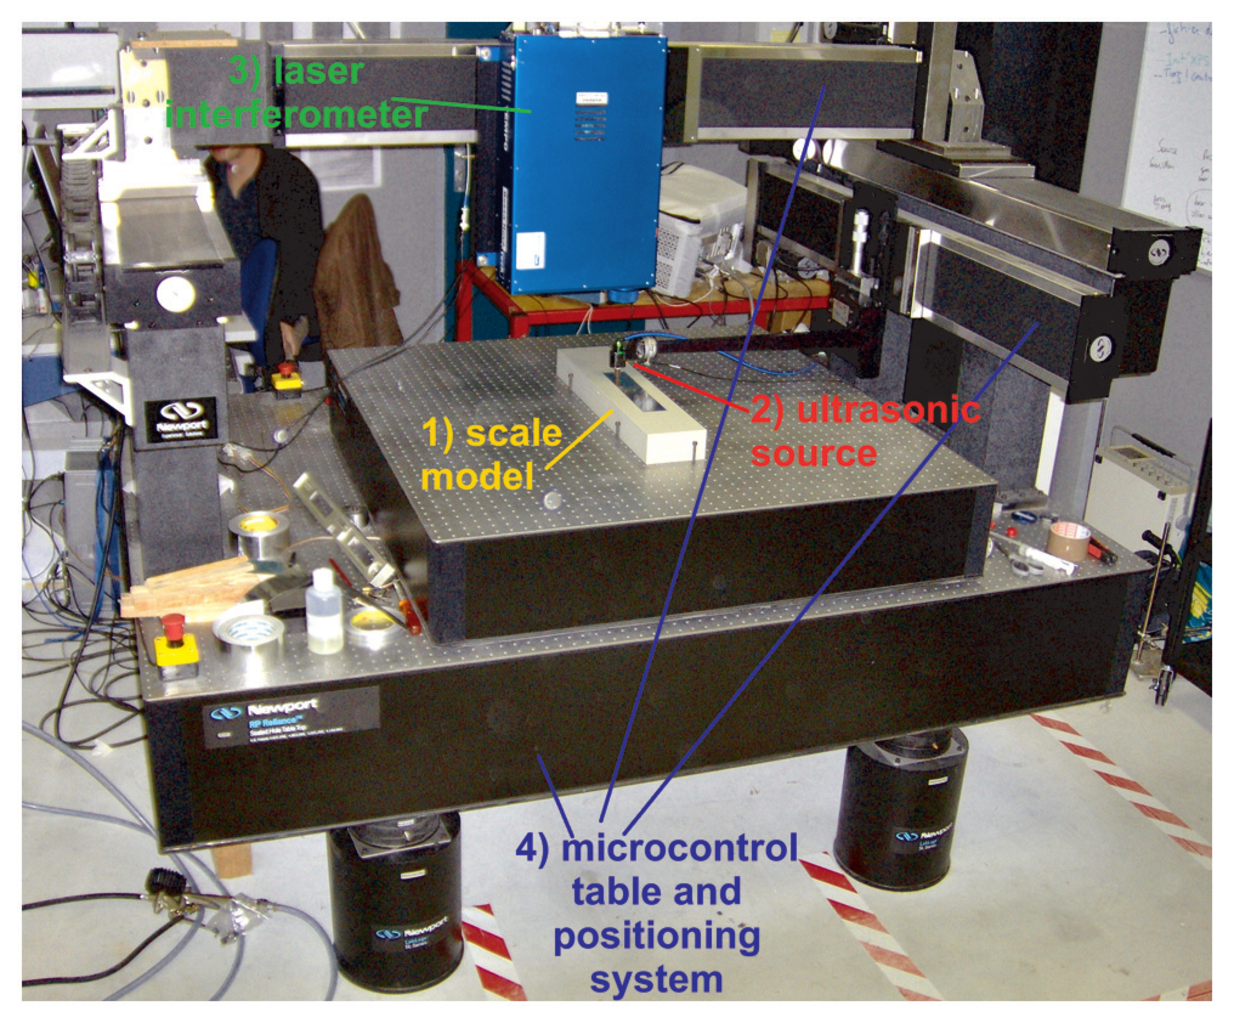
\includegraphics[width=0.75\textwidth]{fig/panel_musc_bench.eps}
	\caption{Photograph of the MUSC ultrasonic laboratory (from \citet{Bretaudeau_FWI_2013} )with its four components: (1) a small-scale model of the underground, (2) an optical table with two automated arms moving above the model, (3) a laser interferometer recording ultrasonic wave propagation	at the model surface,(4) a piezoelectric ultrasonic source generating ultrasonic waves in the model.}
	\label{panel_musc_bench}
\end{figure}

% #### Fig:: panl_multisrcrec
\begin{figure}[!h]
	\centering
	\includegraphics[width=0.75\textwidth]{fig/panel_multisrcrec.eps}
	\caption{Example of multi-source multi-receiver record on the MUSC system for a two-layer model (\bialt).}
	\label{panel_multisrcrec}
\end{figure}

\begin{figure}[!h]
	\centering
	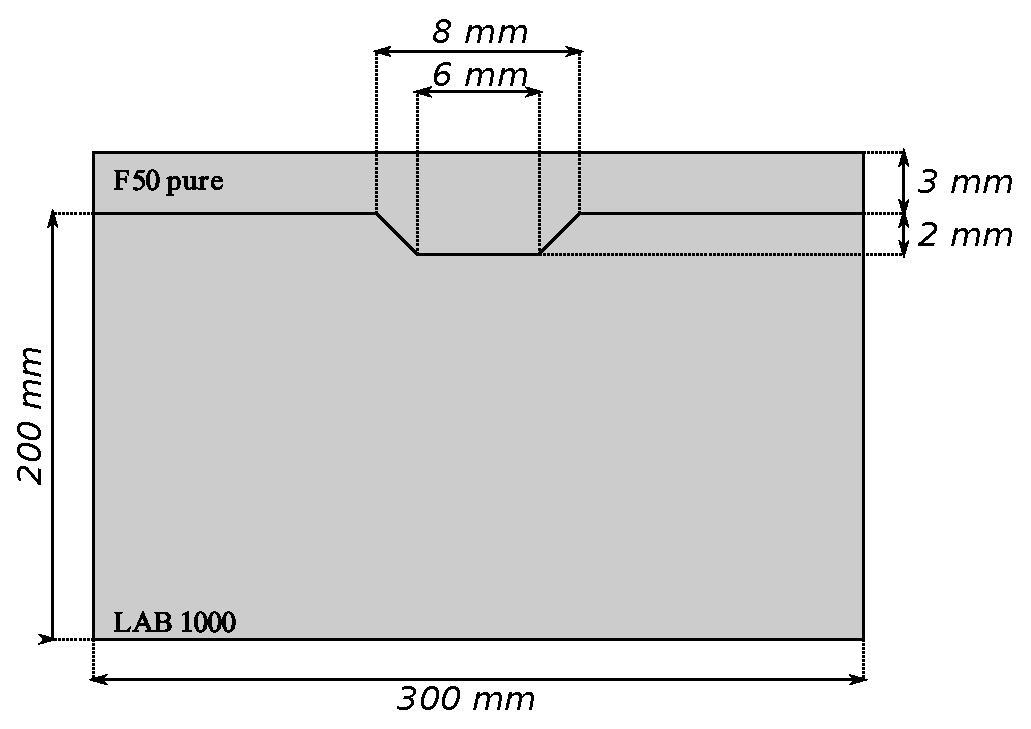
\includegraphics[width=0.75\textwidth]{fig/bialt_model.eps}
	\caption{Schematic representation of the so-called \bialt model.}
	\label{panel_bialt_model}
\end{figure}

\begin{figure}[!h]
	\centering
	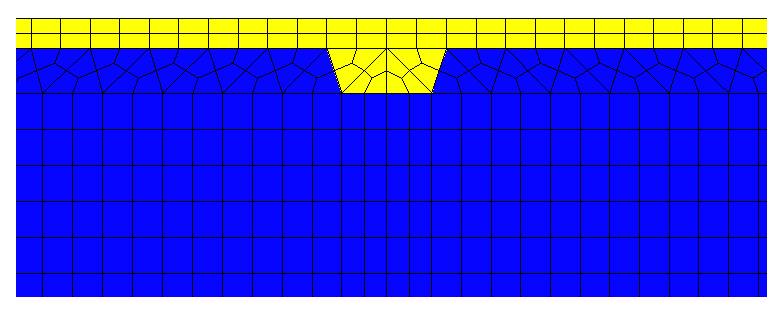
\includegraphics[width=0.75\textwidth]{fig/bialt-mesh.eps}
	\caption{Zoom in the mesh of the \bialt model used for numerical modeling.}
	\label{panel_bialt_mesh}
\end{figure}

% #### Fig:: panel_bialt_2d3d
\begin{figure}[!h]
	\centering
	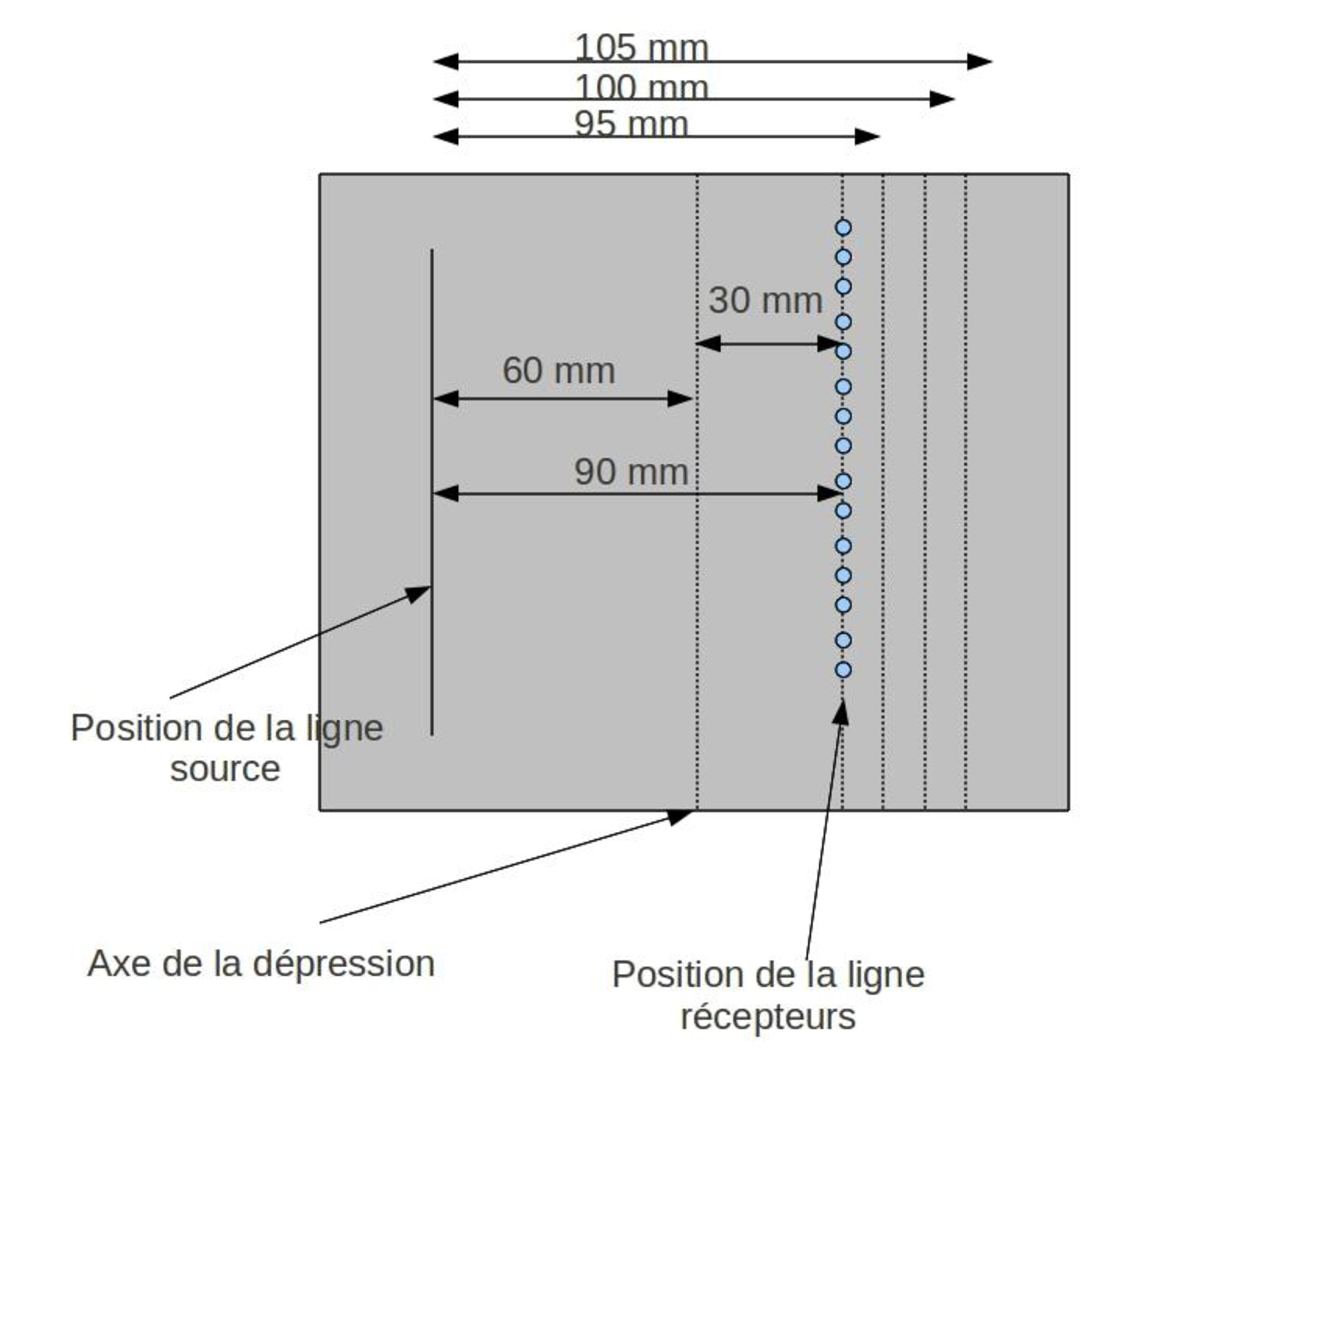
\includegraphics[width=0.75\textwidth]{fig/amplitude_acqui_principle.eps}
	\caption{Schematic representation of the acquisition geometry used to generate experimental line-source, \textit{i.e.} an equivalent of cylindrical source use in two-dimensional modeling. Black traingle and red circle represent receivers and sources, respectively.}
	\label{amplitude_acqui_principle}
\end{figure}

\begin{figure}[!h]
	\centering
	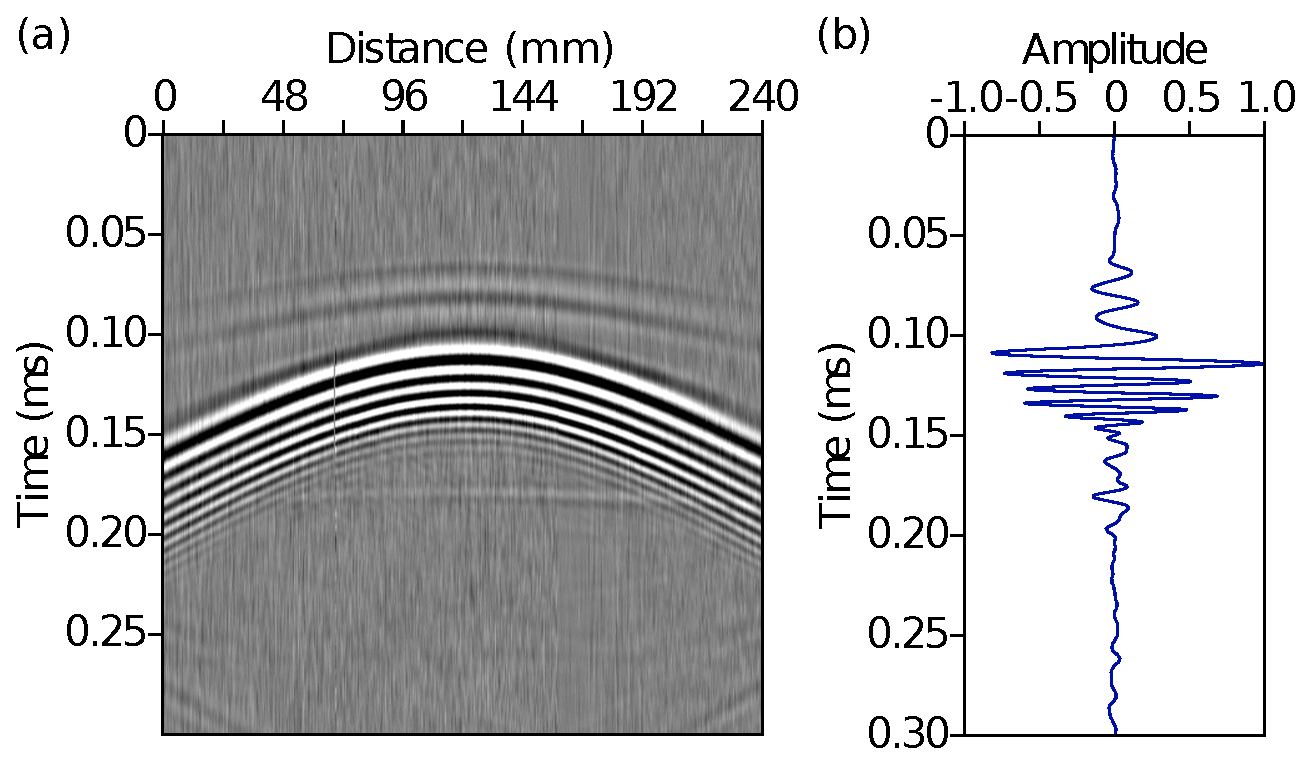
\includegraphics[width=0.75\textwidth]{fig/amplitude_stack_principle.eps}
	\caption{(a,b) Numerical modeling. (a) Resulting seismogram at one receiver position for the experimental line-source. (b) Comparison between point-source response in red (central trace of (a)) , weighted stack response of(a) in green and line-source response from \twod modeling in blue. (c,d) Same as (a) and (b) but for experimental modeling.}
	\label{amplitude_stack_principle}
\end{figure}

\begin{figure}[!h]
	\centering
	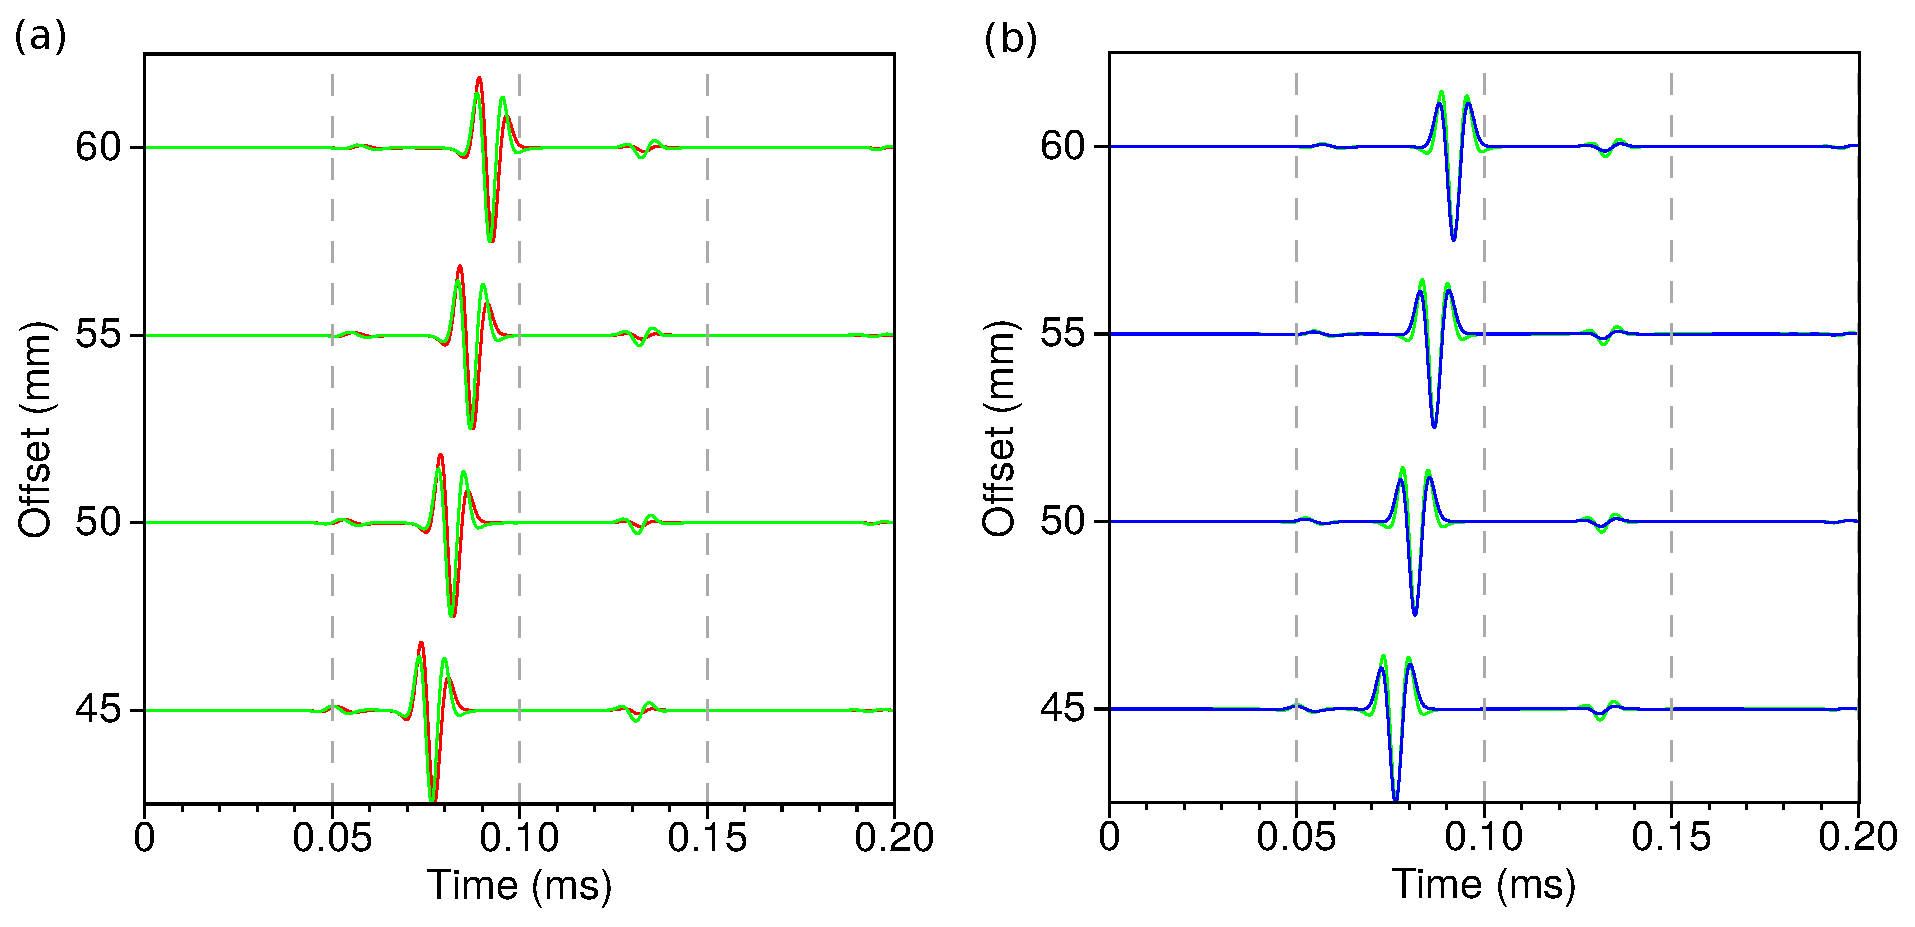
\includegraphics[width=0.75\textwidth]{fig/trans2d3d.eps}
	\caption{(a,b) Numerical modeling. (a) Comparison between synthetic seismograms for a point-source (red) and for a line source (green), for 45, 50, 55 and 60 mm source-receiver offsets respectively. (b) Comparison between synthetic seismograms for a line-source (green), and a point-source response corrected from geometrical spreading (blue) for same source-receiver offsets as (a) using the hybrid method with ratios $r=0.35$, $r=0.40$, $r=0.45$ and $r=0.50$ for offsets $45$, $50$, $55$ and $60\ mm$, respectively . (c,d) Same as (a) and (b) for experimental modeling. The light-purple dotted lines pick $PSv$-wavefront.}%\textbf{cc} gives the correlation factor between line-source and point-source responses.}
	\label{panel_amplitude_sem}
\end{figure}

% #### Fig:: panel_srcest_2d_mean
\begin{figure}[!h]
	\centering
	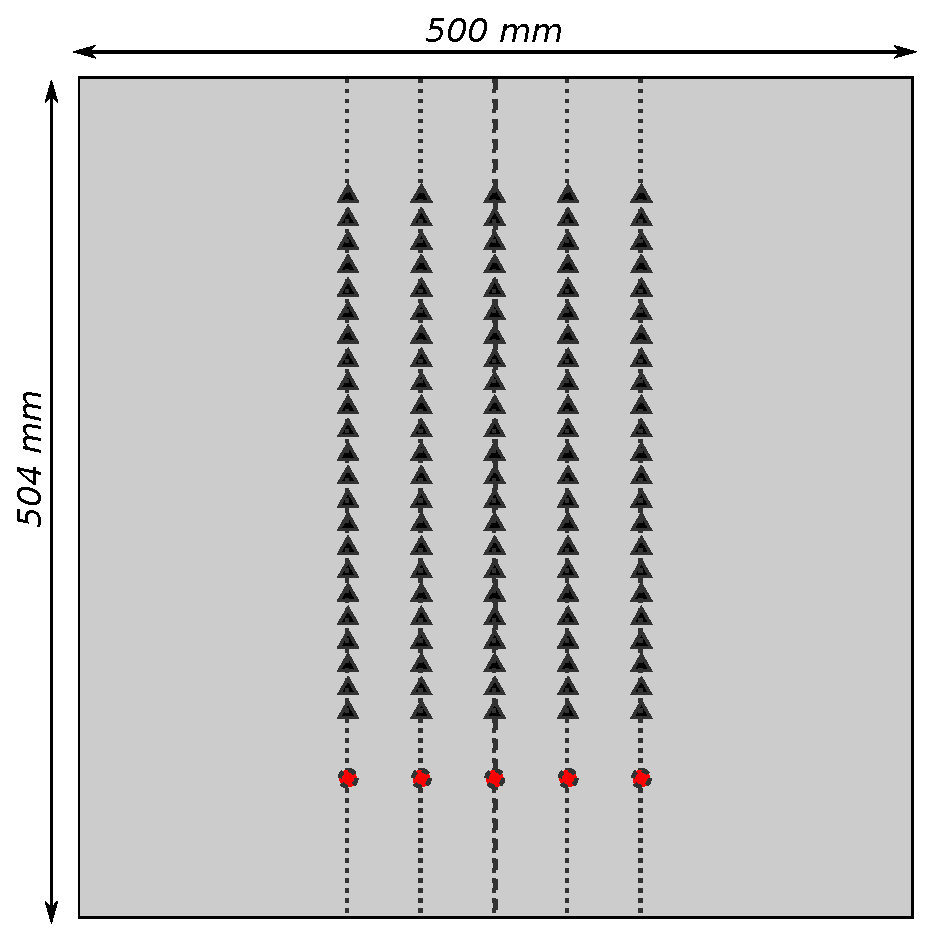
\includegraphics[width=0.75\textwidth]{fig/reproducibility_acqui_principle.eps}
	\caption{Schematic representation of the acquisition geometry used to assess the data reproducibility using the MUSC system. Black traingle and red circle represent receivers and sources, respectively.}
	\label{reproducibility_acqui_principle}
\end{figure}

\begin{figure}[!h]
	\centering
	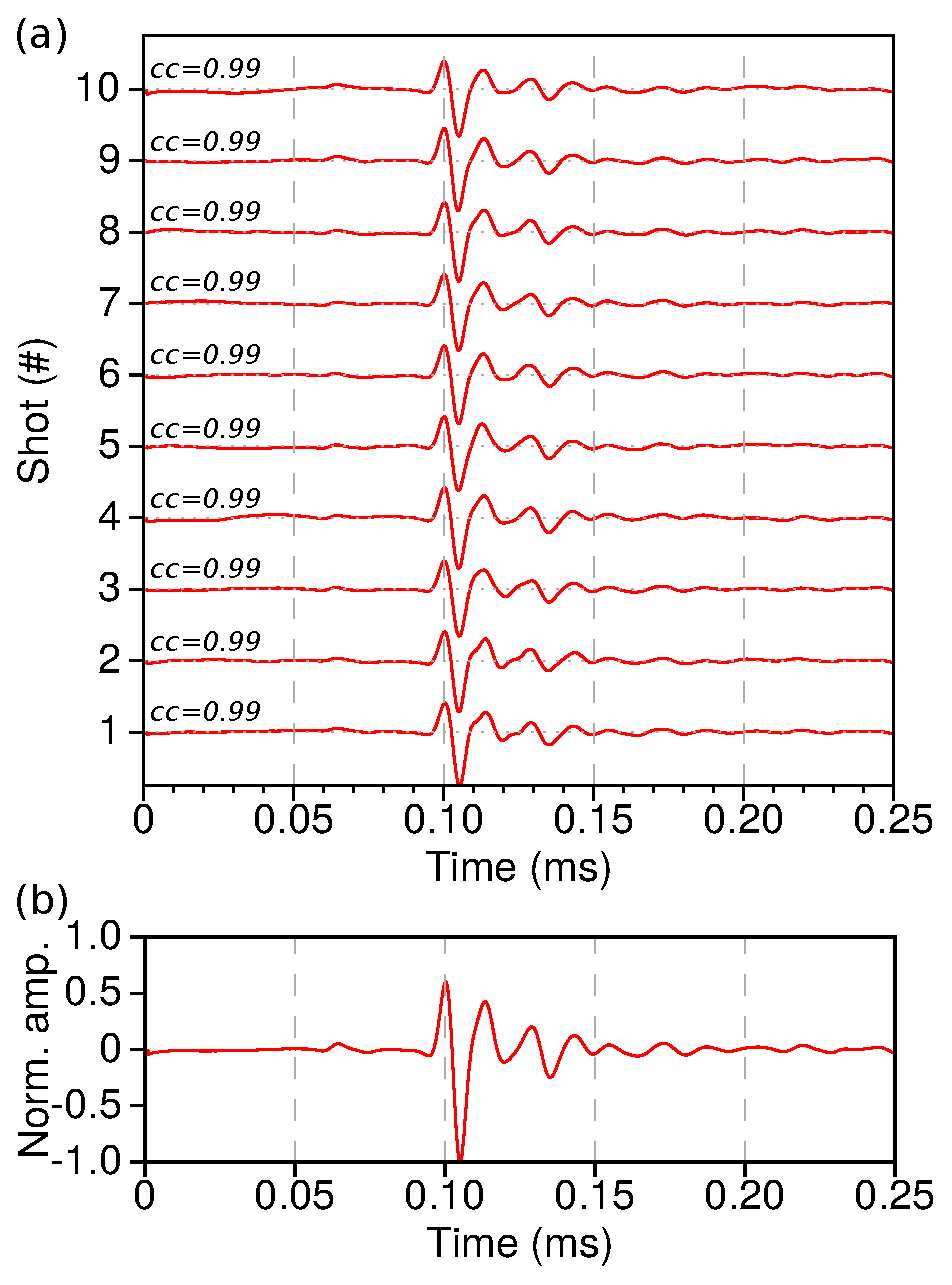
\includegraphics[width=0.75\textwidth]{fig/musc_F50_CT.eps}
	\caption{Central trace for each of the ten analogic experiment compared to a mean central trace (green). \textbf{cc} gives the correlation coefficient between the compared traces.}
	\label{panel_central_traces_cc}
\end{figure}

\begin{figure}[!h]
	\centering
	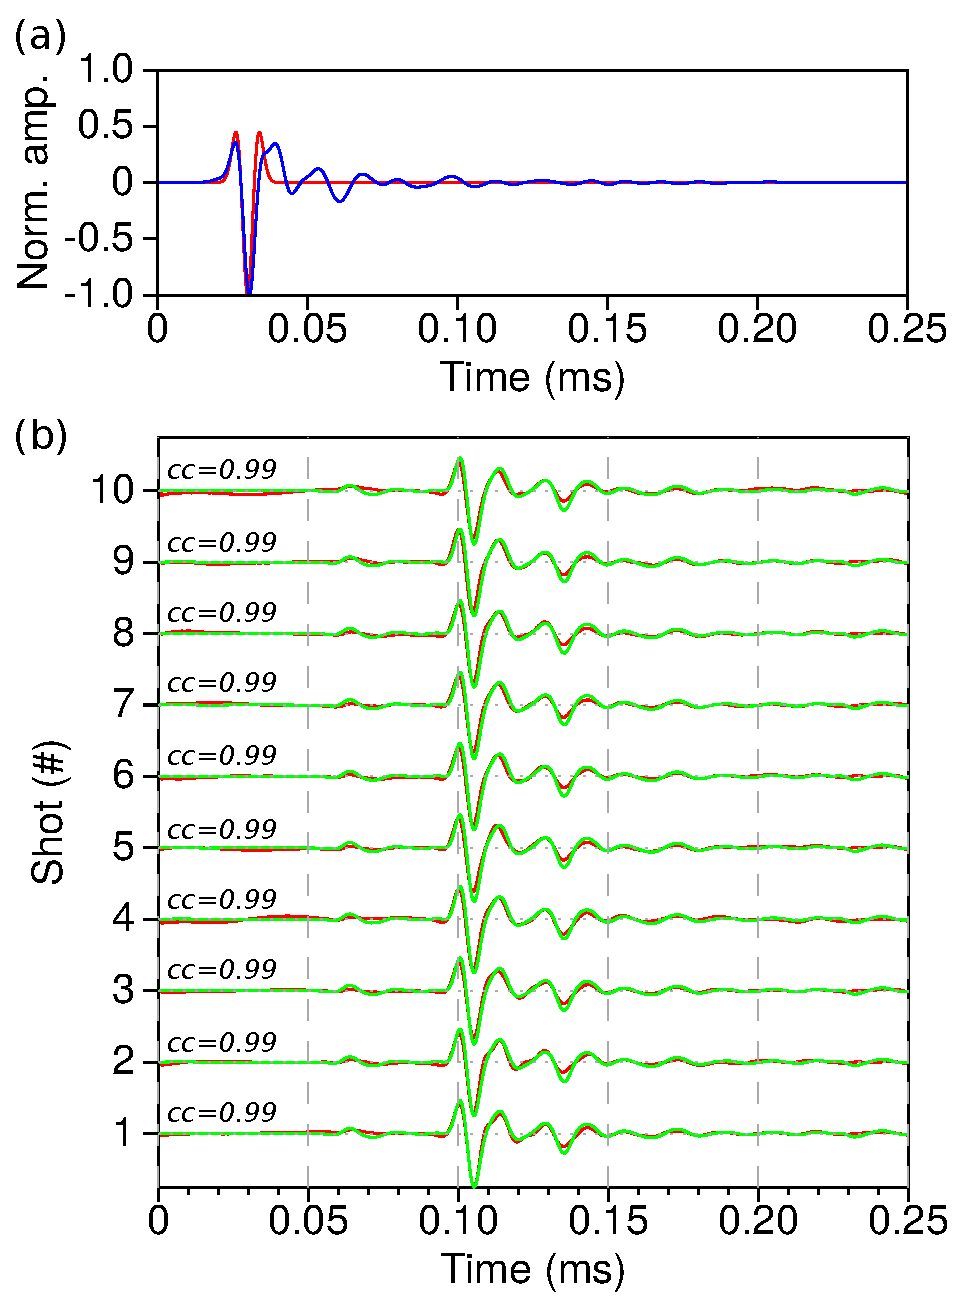
\includegraphics[width=0.75\textwidth]{fig/spec_F50_CT_COMP.eps}
	\caption{(a) Comparison between theoretical Ricker source ($f_{0}=100\ kHz$, $t_{0}=0.03\ ms$) send to the piezo-electric transducer (dashed red line) and the effective source for the homogeneous \textit{F50 pure} model (blue line). (b) Comparison between experimental central traces and numerical ones using the effective source instead theoretical one. \textbf{cc} gives the correlation coefficient between experimental and synthetic traces.}
	\label{panel_srcest_2d_mean_comp}
\end{figure}

% #### Fig:: panel_bialt_model


\begin{figure}[!h]
	\centering
	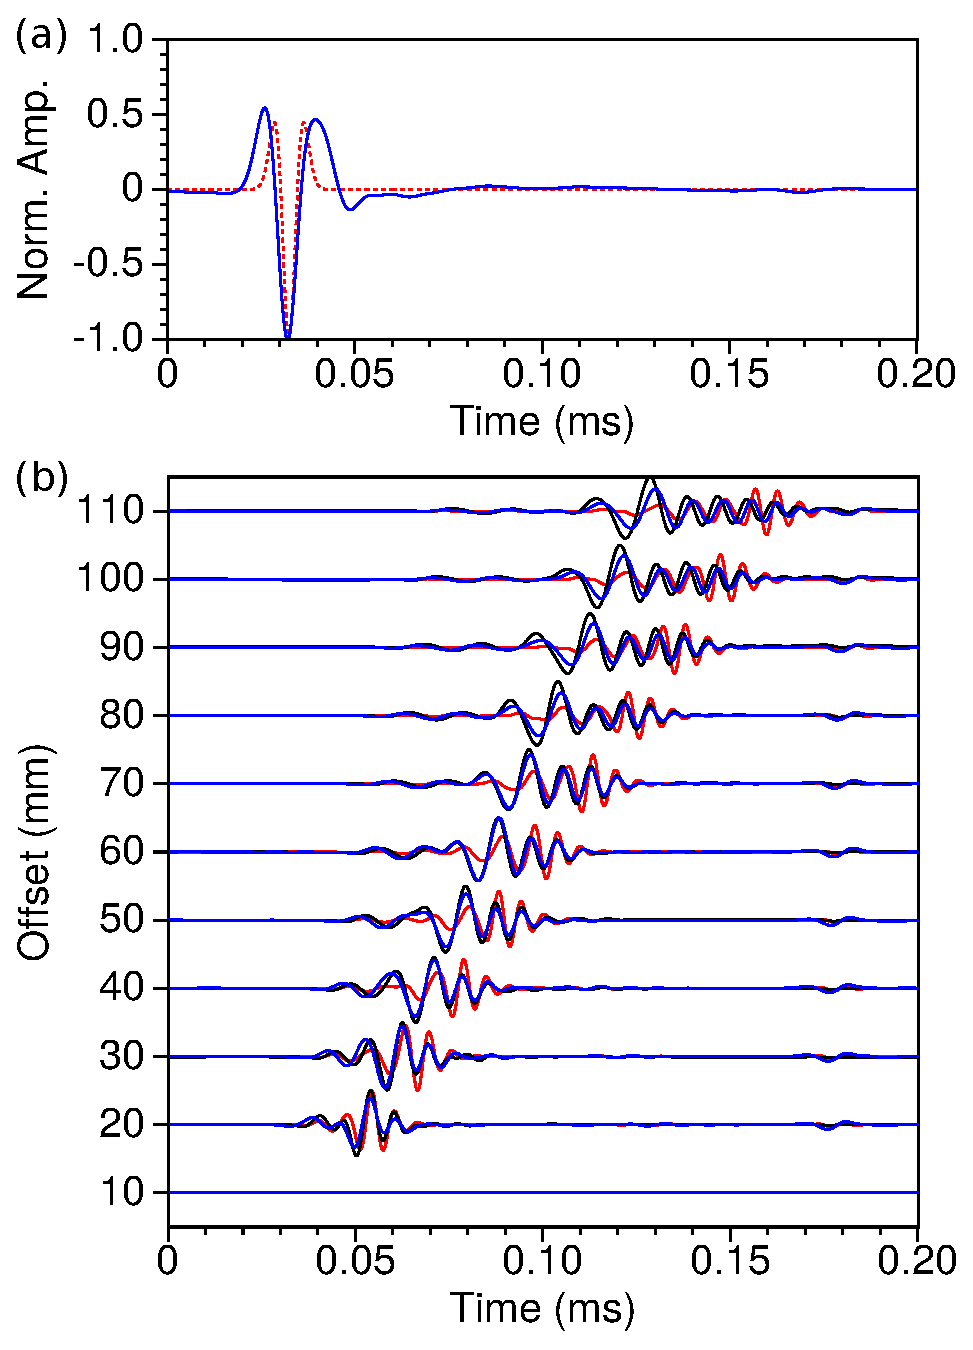
\includegraphics[width=0.75\textwidth]{fig/panel_bialt_lswe.eps}
	\caption{(a) Comparison between theoretical Ricker source ($f_{0}=75\ kHz$, $t_{0}=0.03\ ms$) send to the piezo-electric transducer (dashed red line) and the effective source for the \bialt model (blue line). (b) Comparison between experimental central traces (black), numerical traces using theretical source (red) and numerical traces using the effective source (blue). }
	\label{blind-test}
\end{figure}

\clearpage
\newpage

\subsection*{Tables}

\begin{table}[!ht]
	\centering
	\begin{tabular}{cccccc}
		\hline
		material & Field experiment scale & MUSC experiment scale & scales ratio  \\
		\hline
		P waves velocity & $\mathrm{V_{p 0}}$ & $\mathrm{V_{p 0}}$  & 1  \\
		S waves velocity & $\mathrm{V_{s 0}}$ &  $\mathrm{V_{s 0}}$ & 1   \\
		Time & $\mathrm{T_{0}}$    & 0.001 $\mathrm{T_{0}}$ & 0.001  \\
		frequency   & $\mathrm{F_{0}}$  & 1000 $\mathrm{F_{0}}$ & 1000  \\
		Distance   & $\mathrm{D_{0}}$  & 0.001 $\mathrm{D_{0}}$ & 0.001   \\
		Wavelengh   & $\mathrm{D_{0}}$ & 0.001 $\mathrm{D_{0}}$ & 0.001  \\
		\hline
	\end{tabular}
	\caption{ example of possible scales ratio between field experiments and MUSC experiments when considering a ratio equal to 1 for the density and Quality factor.}
	\label{epoxy-resin}
\end{table}

\begin{table}[!ht]
	\centering
	\begin{tabular}{cccccc}
		\hline
		material & Field experiment scale & MUSC experiment scale & scales ratio  \\
		\hline
		P waves velocity & $\mathrm{V_{p 0}}$ & $\mathrm{2V_{p 0}}$  & 2  \\
		S waves velocity & $\mathrm{V_{s 0}}$ &  $\mathrm{2V_{s 0}}$ & 2   \\
		Time & $\mathrm{T_{0}}$    & 0.001 $\mathrm{T_{0}}$ & 0.001  \\
		frequency   & $\mathrm{F_{0}}$  & 2000 $\mathrm{F_{0}}$ & 2000  \\
		Distance   & $\mathrm{D_{0}}$  & 0.001 $\mathrm{D_{0}}$ & 0.001   \\
		Wavelengh   & $\mathrm{D_{0}}$ & 0.001 $\mathrm{D_{0}}$ & 0.001  \\
		\hline
	\end{tabular}
	\caption{ example of possible scales ratio between field experiments and MUSC experiments when considering a ratio equal to 2 for the density and Quality factor.}
	\label{epoxy-resin}
\end{table}


\begin{table}[!ht]
	\centering
	\begin{tabular}{cccccc}
		\hline
		material & $\mathrm{V_{P}\ (m/s)}$ & $\mathrm{V_{S}\ (m/s)}$ & $\mathrm{V_{R}\ (m/s)}$ & $\mathrm{\rho\ (kg/m^{3})}$ & $\mathrm{Q}$ \\
		\hline
		Aluminium & 5630 & 3225 & --   & 2700 & --  \\
		F50 pure  & 2300 & 1030 & 965  & 1300 & 30  \\
		F50 200\% & 2820 & 1425 & 1328 & 1766 & --  \\
		F50 240\% & 2968 & 1496 & 1388 & 1822 & --  \\
		LAB1000   & 2850 & 1400 & 1310 & 1500 & 75  \\
		\hline
	\end{tabular}
	\caption{Physical properties of some materials used to build small scale models. $\mathrm{V_{P}}$, $\mathrm{V_{S}}$ and $\mathrm{V_{R}}$ are the P-wave velocity, S-wave and the Rayleigh wave velocity, respectively. $\rho$ is the density and $\mathrm{Q}$ is the quality factor.}
	\label{epoxy-resin}
\end{table}

% \begin{table}[!ht]
%	\centering
%	\begin{tabular}{|l|lcr|}
%		
%		\hline
%		Distance               & $d_{real}\ (m)$            & $\rightarrow$ & $k^{-1}d_{reduc}\ (mm)$ \\
%		Wavelength             & $\lambda_{real}\ (m)$      & $\rightarrow$ & %$k^{-1}\lambda_{reduc}\ (mm)$ \\
%		Time                   & $t_{real}\ (s)$            & $\rightarrow$ & $k^{-1}t_{reduc}\ (ms)$ \\
%		Velocity               & $V_{real}\ (m.s^{-1})$     & $\rightarrow$ & $V_{reduc}\ (m.s^{-1})$ \\
%		Density                & $\rho_{real}\ (kg.m^{-3})$ & $\rightarrow$ & $\rho_{reduc}\ (kg.m^{-3})$ \\
%		Quality factor         & $Q_{real}$                 & $\rightarrow$ & $Q_{reduc}$ \\
%		Particule displacement & $a_{real}\ (m)$            & $\rightarrow$ & $k^{-1}a_{reduc}\ (mm)$ \\
%		Particule velocity     & $c_{real}\ (m.s^{-1})$     & $\rightarrow$ & $c_{reduc}\ (m.s^{-1})$ \\
%		\hline
%	\end{tabular}

%	\caption{Scale ratio between viscoelastic parameters at the real scale and at a scale reduced by a coefficient $k$ (after \citet{Bretaudeau_SSM_2011}).}
%	\label{scale-ratio}
%\end{table}

%\begin{table}[!ht] 
%	\centering
%	\begin{tabular}{lcccc}
%		\hline
%		\qquad & 90 mm & 95 mm & 100 mm & 105 mm \\
%		\hline
%		$cc1_{init}$  & 0.702 & 0.725 & 0.728 & 0.728 \\
%		$rms1_{init}$ & 0.794 & 0.760 & 0.762 & 0.774 \\
%		\hline
%		$cc1_{final}$  & 0.940 & 0.953 & 0.951 & 0.949 \\
%		$rms1_{final}$ & 0.358 & 0.317 & 0.325 & 0.343 \\
%		\hline
%		\hline
%		$cc2_{init}$  & 0.954 & 0.987 & 0.988 & 0.988 \\
%		$rms2_{init}$ & 0.304 & 0.162 & 0.155 & 0.154 \\
%		\hline
%		$cc2_{final}$  & --   & --    & --    & --    \\
%		$rms2_{final}$ & --   & --    & --    & --    \\
%		\hline
%	\end{tabular}
%	\caption{.}
%	\label{cc-rms}
%\end{table}

\clearpage
\newpage

\bibliographystyle{seg}  % style file is seg.bst
%\bibliography{/media/pageotd/1581-58C8/Work/git-repository//TR-VIBRIS/tail/bibvibris}
\bibliography{bibvibris,bibvibris_Dona,bibvibris-Dona,references}

\end{document}
